\cleardoublepage

\section{预备知识}
在本节,我们将首先给出一些符号和定义,这些符号和定义在后文使用将不再解释,然后我们将简单介绍间断伽辽金方法的动机与想法,最后给出后文中采用的两种龙格-库塔法,全变差不增龙格-库塔法和隐式-显式龙格-库塔法。
\subsection{基础符号}
本文中我们考虑一维模型并假设计算域为$[a,b]$,首先定义$[a,b]$的一个剖分
\begin{align*}
    I_{j} = (x_{j-1/2}, x_{j+1/2}), \ j = 1, 2, ..., N
\end{align*}
其中$a=x_{1/2} < x_{3/2}< ...< x_{N+1/2}=b$,N表示网格数。接着定义
\begin{align*}
    \Delta x_j = x_{j+1/2}-x_{j-1/2}, \quad h = \max{\sup_j{\Delta x_j}}, \quad x_j = (x_{j+1/2}+x_{j-1/2})/{2},
\end{align*}
其中$\Delta x_j$表示网格大小,$h$表示网格长度,$x_j$表示网格中点。

网格上有限维计算空间$V_h^k = \{v:v|_{I_j}\in P^k(I_j); 1\leq j\leq N\}$,其中$P^k(I_j)$表示$I_j$上次数不大于$k$的多项式集合。我们的数值解和测试函数都将从$V_h^k$中取得。注意到我们并没有对$V^k_h$中的元素附加额外的条件,因此$V_h^k$中的函数在单元边界节点处不一定是连续的,可以出现跳跃。

为了简化标记,我们分别定义$(u_h)^+_{j+1/2}=u_h(x^+_{j+1/2})$和$(u_h)^-_{j+1/2}=u_h(x^-_{j+1/2})$。此外我们定义$u_h$在单元边界节点$x_{j+1/2}$的跳跃$[u_h]_{j+1/2}=(u_h)^+_{j+1/2}-(u_h)^-_{j+1/2}$和均值$(\overline{u}_h)_{j+1/2}=((u_h)_{j+1/2}^++(u_h)_{j+1/2}^-)/2$。
\subsection{逆性质}
我们会列出一些有限元空间$V_h^k$逆性质\cite{ciarlet1978finite},在之后的误差估计中我们将用到这些结论。
对于任意$v \in V_h^k$,存在与v和h无关的正常数$C_i$使得
\begin{equation}
    ||v_x|| \leq C_1 h^{-1} ||v||, \qquad
    ||v||_{\Gamma_h} \leq C_2 h^{-\frac{1}{2}}||v||, \qquad
    ||v||_{0,\infty} \leq C_3 h^{-\frac{d}{2}}||v||.
\end{equation}
其中d是空间维数。由于我们考虑的是一维模型,因此本文$d=1$。
\subsection{间断伽辽金方法基本理论}

在偏微分方程弱形式的理论研究中,我们有以下事实\cite{sullivan2020brief}:
\begin{itemize}
    \item 许多偏微分方程组没有强解但有弱解
    \item 弱解更容易在线性代数表示
    \item 即使强解存在,证明弱解存在性再说明其具有强解的性质往往比直接找到一个强解要简单
\end{itemize}
而本文中的DD模型和HF模型的强解很难求出,因此我们期望弱化要求,求得一个对于测试函数满足我们真正关心的性质的弱解,这同时也能给我们带来编程上的便利。

求解弱解的想法来源于分布理论:由于偏微分方程组源于物理模型,而我们知道当从实际中提取一个物理模型时,我们往往不需要也难以获得某个精确时间或位置的物理量,而常常采用一小段时间或距离的均值来代替。因此我们处理偏微分方程组时也可以考虑方程的积分。此外考虑实际物理量时只需考虑物理量部分特性,我们也可以只考虑偏微分方程组中未知量与测试函数积分的性质。可以说测试函数正是我们观察物理量的维度。基于这些想法,我们求得弱解的方法是在方程两边乘上测试函数并积分得到弱形式,然后利用数值方法求解弱形式。以
\begin{align}
    u_t + f_x = 0\label{eq:SDG}
\end{align}
为例,我们在\eqref{eq:SDG}两边乘以测试函数$v$并分部积分得到
\begin{equation}
    \int_{I_i}u_t v_h\mathrm{d}x - \int_{I_i}f(u)(v_h)_x\mathrm{d}x+v_hf\bigg|^{x_{i+\frac{1}{2}}}_{x_{i-\frac{1}{2}}}.
\end{equation}
这里$f$需要用到相邻单元的值,为了解决这一问题,我们可以采用数值通量
\begin{equation*}
    \hat{f}_{i+\frac{1}{2}}=\hat{f}(u_h(x^-_{i+\frac{1}{2}},t),u_h(x^+_{i+\frac{1}{2}},t))
\end{equation*}
来代替$f$在单元边界处的值。具体来说,数值通量$\hat{f}$需要满足下列要求:
\begin{enumerate}
    \item 一致性:$\hat{f}(u,u)=f(u)$。
    \item 连续性:$\hat{f}$关于两个变量都是Lipschitz连续的。
    \item 单调性:$\hat{f}$关于第一个变量单增,关于第二个单减。可以记作$\hat{f}(\uparrow,\downarrow)$。
\end{enumerate}
这些性质将保证间断伽辽金法的稳定性。

现在我们得到弱形式。
\begin{equation}
    \int_{I_i}u_t v_h\mathrm{d}x - \int_{I_i}f(u)(v_h)_x\mathrm{d}x+\hat{f}_{i+\frac{1}{2}}v_h(x^-_{i+\frac{1}{2}})-\hat{f}_{i-\frac{1}{2}}v_h(x^+_{i-\frac{1}{2}}) = 0. \label{DG:weakSolution}
\end{equation}
间断伽辽金法的想法就是找到独一无二的数值解$u_h^k\in V_h^k$使得对于任意的测试函数$v \in V_h^k$,弱形式\eqref{DG:weakSolution}都成立。但由于计算空间$V_h^k$在单元边界处不连续,我们的数值解$u_h$无法处理高阶导数。因此对于高阶偏微分方程组,按照上述流程无法整理为形如\eqref{DG:weakSolution}的弱形式,我们需要考虑改进DGM来解决这样的高阶偏微分方程组。
\subsubsection{局部间断伽辽金法}
改进的方法就是局部间断伽辽金法(LDG)。LDG法的想法是引入一个辅助变量来使得含有高阶偏导的PDE降阶为只含一阶导的偏微分方程组,然后在这些一阶偏微分方程组上应用DGM。
\begin{equation}
    u_t = u_{xx}
\end{equation}
令$v = u_x$得到
\begin{align}
    u_t - v_x = 0, \\
    v - u_x = 0.
\end{align}
现在我们可以利用DGM来处理该高阶PDE了。
\subsubsection{限制器}
当DGM处理含有不连续的解的模型时,特别是对于包含强离散的问题,依然存在数值振荡,因此我们引入有限元方法中的限制器来限制震荡,同时保证全变差稳定性。限制器的想法是先对当前时间层的数值解进行一个预处理,然后再更新至下一个时间层。本文将采用一种实际中常用的满足全变差有界(TVB)的改进后的minmod限制器\cite{cockburn1989tvb2}。

对于$I_j$上的解$u_h$,首先定义它的平均值
$$
    \overline{u}_j = \frac{1}{\Delta x_j}\int_{I_j}u_h dx,
$$
然后我们定义
\begin{align}
    \tilde{u}_j = m(u_h(x^-_{j+1/2})-\overline{u}_j, \Delta_+\overline{u}_j, \Delta_-\overline{u}_j), \quad \tilde{\tilde{u}}_j = m(\overline{u}_j-u_h(x^+_{j-1/2}), \Delta_+\overline{u}_j, \Delta_-\overline{u}_j),
\end{align}
其中$\Delta_+$和$\Delta_-$是差分算子,定义为
\begin{align}
    \Delta_+\overline{u}_j = \overline{u}_{j+1}-\overline{u}_{j}, \quad \Delta_-\overline{u}_j = \overline{u}_{j}-\overline{u}_{j-1},
\end{align}
minmod函数$m$定义为
\begin{align}
    m(a_1, ..., a_l) & =
    \begin{cases}
        a_1,                         & |a_1| \leq M                                              \\
        s \min_{1\leq i\leq l}|a_i|, & |a_1| \leq M \text{且}s = sign(a_1) = \cdots = sign(a_l), \\
        0 ,                          & \text{其他},
    \end{cases}
\end{align}
这里面的TVB参数M选择有多种选择方式,本文采用相对简便的一种\cite{cockburn1989tvb3}
\begin{align}
    M = \frac{2}{3}\max_{\Omega}u_{xx},
\end{align}
其中$\Omega$表示$u$所有驻点的附近的集合。
最后我们有
\begin{align}
    u^{(mod)}_h(x^-_{j+1/2}) = \overline{u}_j + \tilde{u}_j, \quad u^{(mod)}_h(x^+_{j-1/2}) = \overline{u}_j - \tilde{\tilde{u}}_j.
\end{align}
上述限制限制器本质上是在满足单元平均值$\overline{u}_j$不变的前提下重新计算单元边界处的值。最终,我们能够得到单元平均值以及左右单元边界的值,因此我们可以唯一求出一个$k\leq 2$的多项式。但是对于$k> 2$的情况需要更复杂的分析,简单地把更二次多项式看作更高次多项式可能会导致损失精度。
\subsection{龙格-库塔法案例}
龙格-库塔法(RK)是一种重要的迭代法。一般的显示龙格-库塔法可以表示为
\begin{equation}
    \begin{aligned}
        u^{(i)} = \sum_{l=0}^{i-1}[\alpha_{i,l}u^{(l)} + \beta_{i,l}\Delta tL(u^{(l)})], \quad i = 1,...,m,
        u^{(0)}=u^n,\quad u^{(m)} = u^{n+1}.
    \end{aligned}
    \label{eq:TVDRK}
\end{equation}

由\parencite{shu1998total},我们有得到
\begin{lemma}
    当$a_{ik} \geq 0, \beta_{ik} \geq 0$时,在时间步长$\Delta t \leq \frac{\beta_{ik}}{\alpha_{ik}} \Delta t_1$的条件下,龙格-库塔法\eqref{eq:TVDRK}满足全变差不增。
\end{lemma}

特别地对于三阶TVD RK法,\parencite{shu1998total}给出了最优形式
\begin{equation}
    \begin{aligned}
        u^{(1)} & = u^n + \Delta t L(u^n),                                                \\
        u^{(2)} & = \frac{1}{2}u^n + \frac{1}{4}u^{(1)} + \frac{1}{4}\Delta L(u^{(1)})),  \\
        u^{n+1} & = \frac{1}{3}u^n + \frac{2}{3}u^{(2)} + \frac{2}{3}\Delta t L(u^{(2)}), \\
        CFL     & = 1.
    \end{aligned}
\end{equation}

在给出本文采用的IMEX格式前,我们首先介绍IMEX格式的基本形式。根据\parencite{calvo2001linearly},考虑常微分系统:
\begin{align}
    \frac{dy}{dt} = Ly(t,y) + N(t,y), \quad y(t_0) = y_0,
\end{align}
其中$y = [y_1, y_2, ..., y_d]^T$,$L$是一个$d\times d$的矩阵,来源于扩散项的空间离散,$N(t,y)$来源于对流项的离散。从时间层$t_n$到时间层$t_{n+1}=t_n+h$,我们的求解过程为:
\begin{align*}
    Y_1     & =y_n,                                                                                                        \\
    Y_i     & = y_n + h(\sum_{j=2}^i a_{i,j}LY_j + \sum_{j=1}^{i-1}\hat{a}_{i,j}N(t_n+hc_j,Y_j)), \quad 2 \leq i \leq s+1, \\
    y_{n+1} & = y_n + h(\sum_{i=2}^{s+1}b_iLY_i+\sum_{i=1}^{s+1}\hat{b}_iN(t_n+hc_i, Y_i)),
\end{align*}
其中$Y_j$是过程量。定义$A = (a_{i,j}), \hat{A} = (\hat{a}_{i,j}), b^T = [0, b_2, ..., b_{s+1}], \hat{b}^T=[\hat{b}_1,...,\hat{b}_{s+1}]$和$c^T_{0, c_2, ..., c_{s+1}}$,然后我们将s阶段IMEX格式表示为Butcher表\autoref{tab:IMEX}:
\begin{table}
    \centering
    \begin{minipage}{0.45\linewidth}
        \centering
        \begin{tabular}{c|c}
            c & A \\
            \hline
              & b
        \end{tabular}
    \end{minipage}
    \begin{minipage}{0.45\linewidth}
        \centering
        \begin{tabular}{c|c}
            c & $\hat{A}$ \\
            \hline
              & b
        \end{tabular}
    \end{minipage}
    \caption{IMEX格式的一般形式}
    \label{tab:IMEX}
\end{table}
在上表中$(A|b)$表示DIRK法,$(\hat{A}|\hat{b})$表示ERK法,二者分别应用于对流项和扩散项。

对于一阶IMEXRK法,考虑向后欧拉和向前欧拉\cite{ascher1997implicitexplicita},它的Butcher表如\autoref{tab:IMEX:1}所示;L-稳定二阶段二阶精度DIRK耦合二阶ERK法\cite{ascher1997implicitexplicita},Butcher表如\autoref{tab:IMEX:2}所示,其中$\gamma=1- \sqrt{2}/2,\delta = 1- 1/(2\gamma)$;三阶精度的四阶段L-稳定对角隐式龙格-库塔(DIRK)耦合四阶段显式龙格-库塔(ERK)法\cite{ascher1997implicitexplicita},它们的Butcher表如\autoref{tab:IMEX:3}所示。
\begin{table}
    \centering
    \begin{minipage}{0.45\linewidth}
        \centering
        \begin{tabular}{c|cc}
            0 & 0 & 0 \\
            1 & 0 & 1 \\
            \hline
              & 0 & 1
        \end{tabular}
    \end{minipage}
    \begin{minipage}{0.45\linewidth}
        \centering
        \begin{tabular}{c|cc}
            0 & 0 & 0 \\
            1 & 1 & 0 \\
            \hline
              & 1 & 0
        \end{tabular}.
    \end{minipage}
    \caption{DIRK耦合ERK得到的二阶IMEX格式。左:向后欧拉;右:向前欧拉。}
    \label{tab:IMEX:1}
\end{table}
\begin{table}
    \centering
    \begin{minipage}{0.45\linewidth}
        \centering
        \begin{tabular}{c|ccc}
            0        & 0 & 0          & 0        \\
            $\gamma$ & 0 & $\gamma$   & $0$      \\
            $1$      & 0 & $1-\gamma$ & $\gamma$ \\
            \hline
                     & 0 & $1-\gamma$ & $\gamma$
        \end{tabular}
    \end{minipage}
    \begin{minipage}{0.45\linewidth}
        \centering
        \begin{tabular}{c|ccc}
            0        & 0        & 0           & 0 \\
            $\gamma$ & $\gamma$ & $0$         & 0 \\
            $1$      & $\delta$ & $1- \delta$ & 0 \\
            \hline
                     & $\delta$ & $1-\delta$  & 0
        \end{tabular}.
    \end{minipage}
    \caption{DIRK耦合ERK得到的二阶IMEX格式。左:DIRK;右:ERK。}
    \label{tab:IMEX:2}
\end{table}



\begin{table}
    \centering
    \begin{minipage}{0.45\linewidth}
        \centering
        \begin{tabular}{c|ccccc}
            0             & 0 & 0              & 0              & 0             & 0             \\
            $\frac{1}{2}$ & 0 & $\frac{1}{2}$  & 0              & 0             & 0             \\
            $\frac{2}{3}$ & 0 & $\frac{1}{6}$  & $\frac{1}{2}$  & 0             & 0             \\
            $\frac{1}{2}$ & 0 & $-\frac{1}{2}$ & $\frac{1}{2}$  & $\frac{1}{2}$ & 0             \\
            1             & 0 & $\frac{3}{2}$  & $-\frac{3}{2}$ & $\frac{1}{2}$ & $\frac{1}{2}$ \\
            \hline
                          & 0 & $\frac{3}{2}$  & $-\frac{3}{2}$ & $\frac{1}{2}$ & $\frac{1}{2}$
        \end{tabular}
    \end{minipage}
    \begin{minipage}{0.45\linewidth}
        \centering
        \begin{tabular}{c|ccccc}
            0             & 0               & 0              & 0             & 0              & 0 \\
            $\frac{1}{2}$ & $\frac{1}{2}$   & 0              & 0             & 0              & 0 \\
            $\frac{2}{3}$ & $\frac{11}{18}$ & $\frac{1}{18}$ & 0             & 0              & 0 \\
            $\frac{1}{2}$ & $\frac{5}{6}$   & $-\frac{5}{6}$ & $\frac{1}{2}$ & 0              & 0 \\
            1             & $\frac{1}{4}$   & $\frac{7}{4}$  & $\frac{3}{4}$ & $-\frac{7}{4}$ & 0 \\
            \hline
                          & $\frac{1}{4}$   & $\frac{7}{4}$  & $\frac{3}{4}$ & $-\frac{7}{4}$ & 0
        \end{tabular}.
    \end{minipage}
    \caption{DIRK耦合ERK得到的三阶IMEX格式。左:DIRK;右:ERK。}
    \label{tab:IMEX:3}
\end{table}

\section{DD模型}

本文采用的DD模型表示为
\begin{align}
    n_t - (\mu En)_x = \tau \theta n_{xx}, \label{eq:DD} \\
    \phi_{xx} = \frac{e}{\epsilon}(n - n_d),  \label{eq:poisson}
\end{align}
其中$x\in(0,1)$,第一个电子浓度方程取周期边界条件,第二个电势方程取Dirichlet边界条件:$\phi(0,t) = 0, \phi(1,t) = v_{bias}$。
在系统\eqref{eq:DD}-\eqref{eq:poisson}中,未知量是电子浓度$n$和电势$\phi$。$m_0$表示电子有效质量,k是玻尔兹曼常数,e是电子电荷,$\mu$代表迁移率,$T_0$是晶格温度,$\tau = \frac{m_0 \mu}{e}$是松弛参数,$\theta = \frac{k}{m_0}T_0$,$\epsilon$是介电常量,$n_d$是一个给定的掺杂函数。

\subsection{TVDRK LDG格式}
取$q = \sqrt{\tau \theta }n_x$,那么\autoref{eq:DD}可以写作
\begin{align}
    n_t - (\mu E n)_x - \sqrt{\tau \theta}q_x & = 0, \label{eq:DD:electronConcentration} \\
    q - \sqrt{\tau \theta}n_x                 & = 0. \label{eq:DD:auxiliaryFunction}
\end{align}
而对于泊松方程,本文直接通过积分得到。

令$E = -\phi_x$表示电势,通过引入辅助变量易证$E$具有周期性\cite{liu2010error}。
在方程\eqref{eq:DD:electronConcentration}-\eqref{eq:DD:auxiliaryFunction}两边分别乘以测试函数$v,w\in V_h^k$,分部积分得到
\begin{align}
     & \int_{I_{j}} n_{t} v d x+\int_{I_{j}}(\mu E n+\sqrt{\tau \theta} q) v_{x} d x                                                                               \nonumber                                      \\
     & \quad-(\mu E n+\sqrt{\tau \theta} q)_{j+\frac{1}{2}} v_{j+\frac{1}{2}}^{-}+(\mu E n+\sqrt{\tau \theta} q)_{j-\frac{1}{2}} v_{j-\frac{1}{2}}^{+}=0,            \label{eq:LDG:n}                             \\
     & \int_{I_{j}} q w d x+\int_{I_{j}} \sqrt{\tau \theta} n w_{x} d x-\sqrt{\tau \theta} n_{j+\frac{1}{2}} w_{j+\frac{1}{2}}^{-}+\sqrt{\tau \theta} n_{j-\frac{1}{2}} w_{j-\frac{1}{2}}^{+}=0, \label{eq:LDG:q} \\
     & E_{x}=-\frac{e}{\varepsilon}\left(n-n_{d}\right) .
\end{align}
将上述方程中的精确解$n, q$和$E$替换为它们在$V_{h}^{k}$中的数值近似解$n_h, q_h$。由于数值解$n_h$和$q_h$在单元边界上不连续性,将单元边界上的项替换为适当的数值通量,我们得到LDG格式:
\begin{align}
     & \int_{I_{j}}\left(n_h\right)_{t} v d x+\int_{I_{j}}\left(\mu E_h n_h+\sqrt{\tau \theta} q_h\right) v_{x} d x      \nonumber                                                                                                                    \\
     & \quad-\left(\mu \widehat{E_h n_h}+\sqrt{\tau \theta} \hat{q}_{h}\right)_{j+\frac{1}{2}} v_{j+\frac{1}{2}}^{-}+\left(\mu \widehat{E_h n_h}+\sqrt{\tau \theta} \hat{q}_{h}\right)_{j-\frac{1}{2}} v_{j-\frac{1}{2}}^{+}=0, \label{eq:DDLDGn}     \\
     & \int_{I_{j}} q_h w d x+\int_{I_{j}} \sqrt{\tau \theta} n_h w_{x} d x-\sqrt{\tau \theta} \hat{n}_{j+\frac{1}{2}}^{h} w_{j+\frac{1}{2}}^{-}+\sqrt{\tau \theta} \hat{n}_{j-\frac{1}{2}}^{h} w_{j-\frac{1}{2}}^{+}=0,            \label{eq:DDLDGq} \\
     & E_h=\int_{0}^{x}-\frac{e}{\varepsilon}\left(n_h-n_{d}\right) d x+E_{0}-v_{\text {bias }},\label{eq:DDLDGE}
\end{align}
其中,$E_{0}=E_h(0)=\int_{0}^{1}\left(\int_{0}^{x} \frac{e}{\varepsilon}\left(n_h-n_{d}\right) d s\right) d x$。这里的“$\hat{}$”项表示数值通量。$\hat{n}_{h}$和$\hat{q}_{h}$选择交替通量,即$\hat{n}_{h}=\left(n_h\right)^{+}$,$\hat{q}_{h}=\left(q_h\right)^{-}$,$\widehat{E_h n_h}$采用上风通量,即$\widehat{E_h n_h}=\max \left(E_h, 0\right)\left(n_h\right)^{+}+\min \left(E_h, 0\right)\left(n_h\right)^{-}$。

从LDG格式可知,只要有m时间层的信息,我们可以仅从\eqref{eq:DDLDGq}求得辅助变量$q$,进而求得$m+1$时间层的数值解。这种只需要系统中一个方程求得辅助变量,因此我们这种方法为“局部”间断伽辽金法。这也是与过去需要全局系统才能求出$q$的方法的不同之处。

对于时间离散,我们采用三阶全变差不增(TVD)龙格库塔法。
\begin{align}
    u^{(1)} & = u^n + \Delta t L(u^n),                                                \\
    u^{(2)} & = \frac{3}{4}u^n + \frac{1}{4}u^{(1)} + \frac{1}{4}\Delta t L(u^{(1)}), \\
    u^{n+1} & = \frac{1}{3}u^n + \frac{2}{3}u^{(2)} + \frac{2}{3}\Delta t L(u^{(2)}).
\end{align}
该方法保证$TV(u^{n+1})\leq TV(u^n)$,其中$TV(u) = \sum_j |u_{j+1}-u_j|$。
\subsection{IMEX全离散LDG格式}
本小节,我们将考虑LDG空间离散耦合IMEX时间离散格式。这种IMEX时间离散的想法是显式处理二阶非线性对流项和隐式处理线性扩散项,来减弱对两项都使用显式时间离散所要求的严格的时间步长。这样做可以大量节省我们的算力,同时保持无条件稳定性。

与讨论TVDRK时间离散相比,对于电子浓度方程\eqref{eq:DD},我们有相同的弱形式。而对于泊松方程\eqref{eq:poisson},与TVDRK格式中直接积分不同的是,我们在此处也对它进行空间离散,即对于电势方程组:
\begin{align}
    E_x & = -\frac{e}{\epsilon}(n-n_d), \label{eq:poisson:1} \\
    E   & = - \phi_x. \label{eq:poisson:2}
\end{align}
在等式\eqref{eq:poisson:1}-\eqref{eq:poisson:2}两边分别乘上测试函数$r,z\in V^k_h$得到
\begin{align}
     & -\int_{I_j}Er_x\rm{d}x + E_{j+\frac{1}{2}}r_{j+\frac{1}{2}}^- - E_{j-\frac{1}{2}}r_{j-\frac{1}{2}}^+ = -\frac{e}{\epsilon}\int_{I_j}(n-n_d)r\rm{d}x,                                       \label{DD:weakform:E} \\
     & \int_{I_j} Ez \rm{d}x - \int_{I_j}\phi z_x \rm{d}x + \phi_{j+\frac{1}{2}}z_{j+\frac{1}{2}}^- - \phi_{j-\frac{1}{2}}z_{j-\frac{1}{2}}^+ = 0, \label{DD:weakform:phi}
\end{align}
将单元边界的量替换为对应的数值通量,结合电子浓度方程的LDG格式\eqref{eq:DDLDGn}-\eqref{eq:DDLDGq},我们得到另一种LDG格式:
\begin{align}
     & \int_{I_{j}}\left(n_h\right)_{t} v d x+\int_{I_{j}}\left(\mu E_h n_h+\sqrt{\tau \theta} q_h\right) v_{x} d x      \nonumber                                                                                                                       \\
     & \quad-\left(\mu \widehat{E_h n_h}+\sqrt{\tau \theta} \hat{q}_{h}\right)_{j+\frac{1}{2}} v_{j+\frac{1}{2}}^{-}+\left(\mu \widehat{E_h n_h}+\sqrt{\tau \theta} \hat{q}_{h}\right)_{j-\frac{1}{2}} v_{j-\frac{1}{2}}^{+}=0, \label{eq:IMEX:DD:n}     \\
     & \int_{I_{j}} q_h w d x+\int_{I_{j}} \sqrt{\tau \theta} n_h w_{x} d x-\sqrt{\tau \theta} \hat{n}_{j+\frac{1}{2}}^{h} w_{j+\frac{1}{2}}^{-}+\sqrt{\tau \theta} \hat{n}_{j-\frac{1}{2}}^{h} w_{j-\frac{1}{2}}^{+}=0,            \label{eq:IMEX:DD:q} \\
     & -\int_{I_j}E_hr_x\rm{d}x + (\hat{E}_h)_{j+\frac{1}{2}}r_{j+\frac{1}{2}}^- - (\hat{E}_h)_{j-\frac{1}{2}}r_{j-\frac{1}{2}}^+ = -\frac{e}{\epsilon}\int_{I_j}(n_h-n_d)r\rm{d}x,                                        \label{eq:IMEX:poisson:1}     \\
     & \int_{I_j} E_hz \rm{d}x - \int_{I_j}\phi_h z_x \rm{d}x + (\hat{\phi}_h)_{j+\frac{1}{2}}z_{j+\frac{1}{2}}^- - (\hat{\phi}_h)_{j-\frac{1}{2}}z_{j-\frac{1}{2}}^+ = 0,\label{eq:IMEX:poisson:2}
\end{align}
其中$j = 1,...,N$,带“$\widehat{\ }$”的项是数值通量。我们选择数值通量$\widehat{E_h n_h} = \frac{1}{2}((E_hn_h)^+  + (E_hn_h)^-)$,$\hat{n}_h$和$\hat{q}_h$选择交替通量,即
\begin{equation}
    \hat{n}_h = (n_h)^+, \hat{q}_h = (q_h)^- \quad \text{or} \quad \hat{n}_h = (n_h)^-, \hat{q}_h = (q_h)^+, \label{numbericalFlux:n&q}
\end{equation}
对$\hat{\phi}_h$和$\hat{E}_h$选择带边界条件的交替通量,即
\begin{equation}
    \begin{aligned}
        (\hat{\phi}_h)_{\frac{1}{2}} = (\phi_h^-)_{\frac{1}{2}} = 0, (\hat{\phi}_h)_{j-\frac{1}{2}} = (\phi_h^+)_{j-\frac{1}{2}},j = 2,\cdots,N,(\hat{\phi}_h)_{N-\frac{1}{2}} = (\phi_h^+)_{N-\frac{1}{2}} = v_{bias}, \\
        (\hat{E_h})_{\frac{1}{2}} = (E_h^+)_{\frac{1}{2}} + c_0[\phi]_{\frac{1}{2}}, (\hat{E}_h)_{j-\frac{1}{2}} = (E_h^-)_{j-\frac{1}{2}} + c_0[\phi]_{j-\frac{1}{2}},j = 2,\cdots,N+1,
    \end{aligned}\label{numbericalFlux:phi&E}
\end{equation}
或
\begin{equation}
    \begin{aligned}
        (\hat{\phi}_h)_{\frac{1}{2}} = (\phi_h^-)_{\frac{1}{2}} = 0, (\hat{\phi}_h)_{j-\frac{1}{2}} = (\phi_h^-)_{j-\frac{1}{2}},j = 2,\cdots,N,(\hat{\phi}_h)_{N-\frac{1}{2}} = (\phi_h^+)_{N-\frac{1}{2}} = v_{bias}, \\
        (\hat{E_h})_{j - \frac{1}{2}} = (E_h^+)_{j - \frac{1}{2}} + c_0[\phi]_{j-\frac{1}{2}},j = 2,\cdots,N, (\hat{E}_h)_{N+\frac{1}{2}} = (E_h^-)_{N+\frac{1}{2}} + c_0[\phi]_{N+\frac{1}{2}}.
    \end{aligned}\label{numbericalFlux:phi&E:alt}
\end{equation}
在数值模拟中我们选择第一种。
\subsubsection{一阶IMEX LDG格式}
为了简化表达,我们定义辅助算子
\begin{align}
     & H_j(E_h,n_h,v)    = - (\mu E_h n_h, v_x)_{I_j} + (\mu \hat{E_h n_h})_{j+\frac{1}{2}}v_{j+\frac{1}{2}}^- - (\mu \hat{E_h n_h})_{j-\frac{1}{2}}v_{j-\frac{1}{2}}^+, \label{eq:IMEX:DD:notation:1}                                        \\
     & H_j^{\pm}(u_h,v)  =- \sqrt{\tau \theta}(u_h,v_x)_{I_j} + \sqrt{\tau\theta}(u_h^{\pm})_{j+\frac{1}{2}}v_{j+\frac{1}{2}}^0 - \sqrt{\tau\theta}(u_h^{\pm})_{j-\frac{1}{2}}v_{j-\frac{1}{2}}^+,\quad u = n,q.\label{eq:IMEX:DD:notation:2}
\end{align}
这些辅助算子将同样应用于二阶和三阶格式。
通过分别对\eqref{eq:IMEX:DD:n}-\eqref{eq:IMEX:DD:q}中的对流项和扩散项使用向前欧拉法和向后欧拉法,我们可以得到最简单的一阶IMEX LGD格式:找到数值解$n_h^{m+1},q_h^{m+1}\in V_h$,使得
\begin{align}
    (\frac{n_h^{m+1} - n_h^m}{\Delta t},v)I_j & = -(\mu E_h^mn_h^m, v_x)I_j + (\mu \hat{E_h^mn_h^m})_{j+\frac{1}{2}}v_{j-\frac{1}{2}}^- - (\mu\hat{E_h^mn_h^m})_{j-\frac{1}{2}}v^+_{j-\frac{1}{2}}                                         \nonumber                 \\
                                              & -(\sqrt{\tau \theta}q_h^{m+1},v_x)_{I_j} + (\sqrt{\tau \theta}\hat{q}_h^{m+1})_{j+\frac{1}{2}}v_{j+\frac{1}{2}}^- - (\sqrt{\tau \theta}\hat{q}_h^{m+1})_{j-\frac{1}{2}}v_{j-\frac{1}{2}}^+,  \label{eq:IMEX:1:first} \\
    (q_h^{m+1},w)_{I_j}                       & = -(\sqrt{\tau \theta}n_h^{m+1},w_x)_{I_j} + (\sqrt{\tau \theta}\hat{n}_h^{m+1})_{j+\frac{1}{2}}w_{j+\frac{1}{2}}^- - (\sqrt{\tau \theta}\hat{n}_h^{m+1})_{j-\frac{1}{2}}w_{j-\frac{1}{2}}^+,
\end{align}
其中$j = 1,\cdots,N;\quad r,z \in V_h$。

电势方程的LDG格式是:找到$E_h^{m},\phi_h^{m} \in V_h$,使得
\begin{align}
    -\int_{I_j} E_h^{m}r_x \rm{d}x + (\hat{E}_h^{m})_{j+\frac{1}{2}}r_{j+\frac{1}{2}}^- - (\hat{E}_h^{m})_{j-\frac{1}{2}}r_{j-\frac{1}{2}}^+ = -\frac{e}{\epsilon}\int_{I_j}(n_h^{m} - n_d) r\rm{d} x, \\
    \int_{I_j} E_h^{m}z \rm{d}x - \int_{I_j} \phi_h^{m}z_x \rm{d}x  + (\hat{\phi}_h^{m})_{j+\frac{1}{2}}z^-_{j+\frac{1}{2}} - (\hat{\phi}_h^{m})_{j-\frac{1}{2}}z_{j-\frac{1}{2}}^+  = 0,\label{eq:IMEX:1:last}
\end{align}
中$j = 1,\cdots,N;\quad r,v \in V_h$并且$l = 0,1, u^{m,0} = u^m$。
\subsubsection{二阶IMEX LDG格式}


将\autoref{tab:IMEX:2}对应的二阶阶IMEX时间离散分别应用到\eqref{eq:IMEX:DD:n}-\eqref{eq:IMEX:DD:q}中得到二阶IMEX LDG格式:找到数值解$n_h^{m+1},q_h^{m+1}\in V_h$,使得
\begin{align}
    (\frac{n_h^{m,1} -n_h^m}{\Delta t},v)_{I_j} & = \gamma H_j(E_h^m,n_h^m,v) + \gamma H_j^-(q_h^{m,1},v),              \label{eq:IMEX:2:first} \\
    (\frac{n_h^{m+1} -n_h^m}{\Delta t},v)_{I_j} & = \delta H_j(E_h^m,n_h^m,v) + (1-\delta)H_j(E_h^{m,1},n_h^{m,1},v) \nonumber                  \\
                                                & +(1-\gamma)H_j^-(q_h^{m,1},v) + \gamma H_j^-(q_h^{m+1},v),                                    \\
    (q_h^{m,l},w)_{I_j}                         & = H_j^+(n_h^{m,l},w), l = 1,2, \quad q_h^{m,2} = q_h^{m+1},
\end{align}
其中$j = 1,\cdots,N;\quad v,w \in V_h$并且$\gamma = 1- \frac{\sqrt{2}}{2},\delta = 1 - \frac{1}{2\gamma}$。

电势方程的LDG格式是:找到$E_h^{m,l},\phi_h^{m,l} \in V_h$,使得
\begin{align}
    -\int_{I_j} E_h^{m,l}r_x \rm{d}x + (\hat{E}_h^{m,l})_{j+\frac{1}{2}}r_{j+\frac{1}{2}}^- - (\hat{E}_h^{m,l})_{j-\frac{1}{2}}r_{j-\frac{1}{2}}^+ = -\frac{e}{\epsilon}\int_{I_j}(n_h^{m,l} - n_d) r\rm{d} x, \\
    -\int_{I_j} E_h^{m,l}z \rm{d}x - \int_{I_j} \phi_h^{m,l}z_x \rm{d}x  + (\hat{\phi}_h^{m,l})_{j+\frac{1}{2}}z^-_{j+\frac{1}{2}} - (\hat{\phi}_h^{m,l})_{j-\frac{1}{2}}z_{j-\frac{1}{2}}^+  = 0, \label{eq:IMEX:2:last}
\end{align}
其中$j = 1,\cdots,N; r,v \in V_h, l = 0,1, u^{m,0} = u^m$。带“$\widehat{\ }$”的项代表数值通量,取值可以取\eqref{numbericalFlux:phi&E}或者\eqref{numbericalFlux:phi&E:alt},在后续的数值算例中,对于所有IMEX格式如未加声明,我们都默认取前者。

\subsubsection{三阶IMEX LDG格式}
将\autoref{tab:IMEX:3}对应的三阶IMEX时间离散分别应用到\eqref{eq:IMEX:DD:n}-\eqref{eq:IMEX:poisson:2}中得到三阶IMEX LDG格式:找到数值解$n_h^{m+1}, q_h^{m+1}\in V_h^k$使得
\begin{align}
    (\frac{n_h^{m,1} -n_h^m}{\Delta t},v)_{I_j} & =\frac{1}{2} H_j(E_h^m,n_h^m,v) + \frac{1}{2} H_j^-(q_h^{m,1},v),           \label{eq:IMEX:DD:LDG:1}                       \\
    (\frac{n_h^{m,2} -n_h^m}{\Delta t},v)_{I_j} & = \frac{1}{18} H_j(E_h^m,n_h^m,v) + \frac{1}{18} H_j(E_h^{m,1},n_h^{m,1},v) \nonumber                                      \\
                                                & + \frac{1}{6} H_j^-(q_h^{m,1},v) + \frac{1}{2} H_j^-(q_h^{m,2},v),                                                         \\
    (\frac{n_h^{m,3} -n_h^m}{\Delta t},v)_{I_j} & =\frac{5}{6} H_j(E_h^m,n_h^m,v) -\frac{5}{6} H_j(E_h^{m,1},n_h^{m,1},v) + \frac{1}{2} H_j(E_h^{m,2},n_h^{m,2},v) \nonumber \\
                                                & - \frac{1}{2} H_j^-(q_h^{m,1},v) + \frac{1}{2} H_j^-(q_h^{m,2},v) + \frac{1}{2} H_j^-(q_h^{m,3},v),                        \\
    (\frac{n_h^{m+1} -n_h^m}{\Delta t},v)_{I_j} & = \frac{1}{4} H_j(E_h^m,n_h^m,v) +\frac{7}{4} H_j(E_h^{m,1},n_h^{m,1},v)  \nonumber                                        \\
                                                & + \frac{3}{4} H_j(E_h^{m,2},n_h^{m,2},v) - \frac{7}{4} H_j(E_h^{m,3},n_h^{m,3},v) \nonumber                                \\
                                                & +\frac{3}{2} H_j^-(q_h^{m,1},v) -\frac{3}{2} H_j^-(q_h^{m,2},v) \nonumber                                                  \\
                                                & + \frac{1}{2} H_j^-(q_h^{m,3},v)  + \frac{1}{2} H_j^-(q_h^{m+1},v),                                                        \\
    (q_h^{m,1},w)_{I_j}                         & = H_j^+(n_h^{m,l},w), l = 1,2,3,4, q_h^{m,4} = q_h^{m+1},\label{eq:IMEX:DD:LDG:4}
\end{align}
其中$j = 1,\cdots,N;v,w \in V_h$,$H_j$和$H_j^{\pm}$定义如\eqref{eq:IMEX:DD:notation:1}-\eqref{eq:IMEX:DD:notation:2}所示。


电势方程的LDG格式是:找到$E_h^{m,l},\phi_h^{m,l} \in V_h$,使得
\begin{align}
    -\int_{I_j} E_h^{m,l}r_x \rm{d}x + (\hat{E}_h^{m,l})_{j+\frac{1}{2}}r_{j+\frac{1}{2}}^- - (\hat{E}_h^{m,l})_{j-\frac{1}{2}}r_{j-\frac{1}{2}}^+ = -\frac{e}{\epsilon}\int_{I_j}(n_h^{m,l} - n_d) r\rm{d} x, \label{eq:IMEX:poisson:LDG:1} \\
    \int_{I_j} E_h^{m,l}z \rm{d}x - \int_{I_j} \phi_h^{m,l}z_x \rm{d}x  + (\hat{\phi}_h^{m,l})_{j+\frac{1}{2}}z^-_{j+\frac{1}{2}} - (\hat{\phi}_h^{m,l})_{j-\frac{1}{2}}z_{j-\frac{1}{2}}^+  = 0,\label{eq:IMEX:poisson:LDG:2}
\end{align}
其中$j = 1,\cdots,N; r,z \in V_h$且$l = 0,1,2,3, u^{m,0} = u^m$,数值通量的选择和之前相同。

\subsection{误差估计}
\subsubsection{DD模型三阶TVD LDG格式}
对于DD模型的三阶TVD LDG格式,我们有以下误差估计\cite{liu2010error}:
\begin{theorem}
    设$n, q$是问题\eqref{eq:DD:electronConcentration}-\eqref{eq:DD:auxiliaryFunction}的精确解,它们足够光滑且有有界导数。设$n^{h}, q^{h}$是半离散LDG格式\eqref{eq:DDLDGn}-\eqref{eq:DDLDGq}的数值解。相应的数值误差记为$e_{u}=u-u_{h}(u=n, q)$。如果有限元空间$V_{h}^{k}$是$k \geq 1$次分段多项式,则对于足够小的$h$,有以下误差估计成立:
    \begin{equation}
        \left\|n-n^{h}\right\|_{L^{\infty}\left(0, T ; L^{2}\right)}+\left\|q-q^{h}\right\|_{L^{2}\left(0, T ; L^{2}\right)} \leq C h^{k+\frac{1}{2}},
    \end{equation}
    其中常数$C$依赖于最终时间$T,k, \|n\|_{L^{\infty}\left(0, T ; H^{k+1}\right)}, \left\|n_{x}\right\|_{0, \infty}和\left\|n_{d}\right\|_{0, \infty}$。
\end{theorem}

\subsubsection{一阶IMEX LDG格式}
我们在关于IMEX LDG格式中我们有定义:$||u||_{L^{\infty}(0,T;L^2)}  = \max \limits_{0 \leq t \leq T}||u^m||_{l^2(I)}$和$||u||_{L^2(0,T;L^2)} = (\int_{0}^{T}||u^m||_{L^2(I)}^2\Delta t)^{1/2}$
对于一阶IMEX LDG格式,我们有以下误差估计\cite{liu2016analysis}:
\begin{theorem}
    令$n^m,q^m$是问题\eqref{eq:LDG:n}-\eqref{eq:LDG:q}和\eqref{DD:weakform:E}-\eqref{DD:weakform:phi}在时间层级m的精确解,它们足够光滑且有有界导数。令$n_h^m,q_h^m$是一阶IMEX LDG格式\eqref{eq:IMEX:1:first}-\eqref{eq:IMEX:1:last}的数值解。如果有限元空间$V_h^k$是k$(k\geq  0)$阶间断多项式,那么对于足够小的h,存在与h无关的正常数C,使得下列误差估计成立
    \begin{equation}
        ||n-n_h||_{L^{\infty}(0,T;L^2)} + ||q - q_h||_{L^2(0,T;L^2)} \leq C(h^{k+1} + (\Delta t)^2), \label{eq:IMEX:es:2}
    \end{equation}
    其中C依赖于最终时间$T,k,C_{\mu}$,反常数$C_2, ||n||_{L^{\infty}(0,T;H^{k+1})}, ||n_x||_{L^{\infty}}$和$||E||_{L^{\infty}}$。
\end{theorem}
\subsubsection{二阶IMEX LDG格式}
对于二阶IMEX LDG格式,我们有以下误差估计\cite{liu2016analysis}:
\begin{theorem}
    令$n^m,q^m$是问题\eqref{eq:LDG:n}-\eqref{eq:LDG:q}和\eqref{DD:weakform:E}-\eqref{DD:weakform:phi}在时间层级m的精确解,它们足够光滑且有有界导数。令$n_h^m,q_h^m$是二阶IMEX LDG格式\eqref{eq:IMEX:2:first}-\eqref{eq:IMEX:2:last}的数值解。如果有限元空间$V_h^k$是k$(k\geq  0)$阶间断多项式,那么对于足够小的h,存在与h无关的正常数C,使得下面的误差估计成立
    \begin{equation}
        ||n-n_h||_{L^{\infty}(0,T;L^2)} \leq C(h^{k+1} + (\Delta t)^2), \label{eq:IMEX:es:2}
    \end{equation}
    其中C依赖于最终时间$T,k,C_{\mu}$,反常数$C_2, ||n||_{L^{\infty}(0,T;H^{k+1})}, ||n_x||_{L^{\infty}}$和$||E||_{L^{\infty}}$。
\end{theorem}
\subsubsection{三阶IMEX LDG格式}
对于三阶IMEX LDG格式,我们有以下误差估计\cite{liu2016analysis}:
\begin{theorem}
    令$n^m,q^m$是问题\eqref{eq:LDG:n}-\eqref{eq:LDG:q}和\eqref{DD:weakform:E}-\eqref{DD:weakform:phi}在时间层级m的精确解,它们足够光滑且有有界导数。令$n_h^m,q_h^m$是三阶IMEX LDG格式\eqref{eq:IMEX:DD:LDG:1} -\eqref{eq:IMEX:DD:LDG:4}。如果有限元空间$V_h^k$是k$(k\geq  0)$阶间断多项式,那么对于足够小的h,存在与h无关的正常数C,使得下面的误差估计成立
    \begin{equation}
        ||n-n_h||_{L^{\infty}(0,T;L^2)} \leq C(h^{k+1} + (\Delta t)^3), \label{eq:IMEX:es:3}
    \end{equation}
    其中C依赖于最终时间$T,k,C_{\mu}$,反常数$C_2, ||n||_{L^{\infty}(0,T;H^{k+1})}, ||n_x||_{L^{\infty}}$和$||E||_{L^{\infty}}$。
\end{theorem}
\section{HF模型}
高场模型由以下方程以及带有周期边界条件的Poisson电场方程~\eqref{eq:poisson}表示
\begin{equation}
    n_{t}+J_{x}=0, \quad x \in(0,1) \label{eq:HF}
\end{equation}
其中
$$
    J=J_{h y p}+J_{v i s}
$$

$$
    \begin{gathered}
        J_{h y p}=-\mu n E+\tau \mu\left(\frac{e}{\varepsilon}\right) n(-\mu n E+\omega) \\
        J_{v i s}=-\tau\left(n\left(\theta+2 \mu^{2} E^{2}\right)\right)_{x}+\tau \mu E(\mu n E)_{x} .
    \end{gathered}
$$
这里,$\omega=\left.(\mu n E)\right|_{x=0}$取常数。
\subsection{TVDRK LDG格式}
未知量与DD模型中相同:电子浓度$n$和电势$\phi$。由于
$$
    -2\left(n E^{2}\right)_{x}+E(n E)_{x}=-3 n E E_{x}-E^{2} n_{x}
$$
上述方程可以写作
\begin{equation}
    n_{t}+\left(-\mu n E-\tau \mu^{2} \frac{e}{\varepsilon} n^{2} E+\tau \mu \frac{e}{\varepsilon} \omega n-3 \tau \mu^{2} E n E_{x}\right)_{x}-\left(\left(\tau \theta+\tau \mu^{2} E^{2}\right) n_{x}\right)_{x}=0.\label{eq:HFRewritten}
\end{equation}
利用$E_{x}=-\frac{e}{\varepsilon}\left(n-n_{d}\right)$,定义$C_{1}=\frac{\tau \mu e}{\varepsilon}$,$C_{2}=\frac{\tau \mu^{2} e}{\varepsilon}=\mu C_{1}$和$C_{3}=\frac{\tau \mu e \omega}{\varepsilon}=\omega C_{1}$,方程~\eqref{eq:HFRewritten}可以简写为
\begin{equation}
    n_{t}+\left(-\left(3 C_{2} E n_{d}+\mu E-C_{3}\right) n+2 C_{2} E n^{2}\right)_{x}-\left(\left(\tau \theta+\tau \mu^{2} E^{2}\right) n_{x}\right)_{x}=0 .  \label{eq:HFRewrittenc}
\end{equation}
设$q=\sqrt{\tau \theta+\tau \mu^{2} E^{2}} n_{x}=\left(\sqrt{\tau \theta+\tau \mu^{2} E^{2}} n\right)_{x}-\left(\sqrt{\tau \theta+\tau \mu^{2} E^{2}}\right)_{x} n$,我们可以将方程$~\eqref{eq:HFRewrittenc}$按照LDG的方法改写为更大的一阶PDE系统
\begin{align}
     & n_{t}+\left(-\left(3 C_{2} E n_{d}+\mu E-C_{3}\right) n+2 C_{2} E n^{2}-\sqrt{\tau \theta+\tau \mu^{2} E^{2}} q\right)_{x}=0, \label{eq:HFRewrittenca} \\
     & q=\left(\sqrt{\tau \theta+\tau \mu^{2} E^{2}} n\right)_{x}-\left(\sqrt{\tau \theta+\tau \mu^{2} E^{2}}\right)_{x} n.\label{eq:HFRewrittencb}
\end{align}
分别用测试函数$v, w \in V_{h}^{k}$乘以方程~\eqref{eq:HFRewrittenca}-\eqref{eq:HFRewrittencb},并对所有涉及空间导数的项分部积分,得到以下弱形式
\begin{align}
     & \int_{I_{j}} n_{t} v d x+\int_{I_{j}}\left(3 C_{2} E n_{d}+\mu E-C_{3}\right) n v_{x} d x                                                                          \nonumber                                              \\
     & -\left(3 C_{2} E n_{d} n+\mu E n-C_{3} n\right)_{j+\frac{1}{2}} v_{j+\frac{1}{2}}^{-}                                                                                       \nonumber                                     \\
     & +\left(3 C_{2} E n_{d} n+\mu E n-C_{3} n\right)_{j-\frac{1}{2}} v_{j-\frac{1}{2}}^{+}                                                                                      \nonumber                                      \\
     & -\int_{I_{j}} 2 C_{2} E n^{2} v_{x} d x+2 C_{2}\left(E n^{2}\right)_{j+\frac{1}{2}} v_{j+\frac{1}{2}}^{-}-2 C_{2}\left(E n^{2}\right)_{j-\frac{1}{2}} v_{j-\frac{1}{2}}^{+}           \nonumber                           \\
     & +\int_{I_{j}} \sqrt{\tau \theta+\tau \mu^{2} E^{2}} q v_{x} d x                                                                                               \nonumber                                                   \\
     & -\left(\sqrt{\tau \theta+\tau \mu^{2} E^{2}} q\right)_{j+\frac{1}{2}} v_{j+\frac{1}{2}}^{-}+\left(\sqrt{\tau \theta+\tau \mu^{2} E^{2}} q\right)_{j-\frac{1}{2}} v_{j-\frac{1}{2}}^{+}=0  \label{eq:HFRewrittenWeakForma} \\
     & \int_{I_{j}} q w d x+\int_{I_{j}} \sqrt{\tau \theta+\tau \mu^{2} E^{2}} n w_{x} d x+\int_{I_{j}}\left(\sqrt{\tau \theta+\tau \mu^{2} E^{2}}\right)_{x} n w d x    \nonumber                                               \\
     & -\left(\sqrt{\tau \theta+\tau \mu^{2} E^{2}} n\right)_{j+\frac{1}{2}} w_{j+\frac{1}{2}}^{-}+\left(\sqrt{\tau \theta+\tau \mu^{2} E^{2}} n\right)_{j-\frac{1}{2}} w_{j-\frac{1}{2}}^{+}=0 .\label{eq:HFRewrittenWeakFormb}
\end{align}
将上述方程中的精确解$n, q$替换为它们在$V_{h}^{k}$中的数值近似$n_h, q_h$。注意到数值解$n_h$和$q_h$在单元边界上不连续,我们需要将单元边界上的项替换为合适的数值通量。为了简化,我们定义$a_h:=\sqrt{\tau \theta+\tau \mu^{2}\left(E_h\right)^{2}}$,$b_h:=3 C_{2} E_h n_{d}+\mu E_h-C_{3}$,最终得到LDG格式:
\begin{align}
     & \int_{I_{j}} n_{t}^{h} v d x+\int_{I_{j}}\left(b_h\right) n_h v_{x} d x                                                                    -\left(b_h\right)_{j+\frac{1}{2}} \hat{n}_{j+\frac{1}{2}}^{h} v_{j+\frac{1}{2}}^{-}  +\left(b_h\right)_{j-\frac{1}{2}} \hat{n}_{j-\frac{1}{2}}^{h} v_{j-\frac{1}{2}}^{+}                                                                                                                                   \nonumber \\
     & -\int_{I_{j}} 2 C_{2} E_h\left(n_h\right)^{2} v_{x} d x+2 C_{2}\left(E_h \widehat{\left(n_h\right)^{2}}\right)_{j+\frac{1}{2}} v_{j+\frac{1}{2}}^{-}-2 C_{2}\left(E_h \widehat{\left(n_h\right)^{2}}\right)_{j-\frac{1}{2}} v_{j-\frac{1}{2}}^{+} \nonumber                                                                                                                                                                                                     \\
     & +\int_{I_{j}} a_h q_h v_{x} d x -\left(a_h \hat{q}_{h}\right)_{j+\frac{1}{2}} v_{j+\frac{1}{2}}^{-}+\left(a_h \hat{q}_{h}\right)_{j-\frac{1}{2}} v_{j-\frac{1}{2}}^{+}=0,             \label{eq:HFRewrittenLDGa}                                                                                                                                                                                                                                                \\
     & \int_{I_{j}} q_h w d x+\int_{I_{j}} a_h n_h w_{x} d x+\int_{I_{j}}\left(a_h\right)_{x} n_h w d x                        \nonumber                                                                                                                                                                                                                                                                                                                               \\
     & -\left(a_h \hat{n}_{h}\right)_{j+\frac{1}{2}} w_{j+\frac{1}{2}}^{-}+\left(a_h \hat{n}_{h}\right)_{j-\frac{1}{2}} w_{j-\frac{1}{2}}^{+}=0 .\label{eq:HFRewrittenLDGb}
\end{align}
数值电场$E_h$的与之前一样直接通过积分来求解。这里的“$\widehat{\ }$”项表示数值通量。$a_h \hat{n}_{h}$和$a_h \hat{q}_{h}$选择交替通量,即$a_h \hat{n}_{h}=a_h\left(n_h\right)^{+}$,$a_h \hat{q}_{h}=a_h\left(q_h\right)^{-}$;对于$b_h \hat{n}_{h}$,我们选择上风通量,即如果$b_h>0$,则$b_h \hat{n}_{h}=b_h\left(n_h\right)^{+}$,否则$b_h \hat{n}_{h}=b_h\left(n_h\right)^{-}$;对于通量$\widehat{\left(n_h\right)^{2}}$,有两种选择:$\widehat{\left(n_h\right)^{2}}=\frac{\left(n^{h-}\right)^{2}+\left(n_h\right)^{-}\left(n_h\right)^{+}+\left(n^{h-}\right)^{2}}{3}$或$\widehat{\left(n_h\right)^{2}}=\frac{\left(n^{h-}\right)^{2}+\left(n_h\right)^{-}\left(n_h\right)^{+}+\left(n^{h-}\right)^{2}}{3}-\alpha\left[n_h\right]$(如果$E_h>0$,则$\alpha=1$;否则$\alpha=-1$)。在本文数值模拟中,我们实现前者。
\subsection{误差估计}
对于HF模型的三阶TVD LDG格式,同样为了简便我们定义$a:=\sqrt{\tau \theta+\tau \mu^{2}\left(E\right)^{2}}, b:=3 C_{2} E n_{d}+\mu E-C_{3}$,然后我们有误差估计\cite{liu2010error}:
\begin{theorem}
    设$n, q$是问题\eqref{eq:HFRewrittenca}-\eqref{eq:HFRewrittencb}的精确解,具有足够光滑且有界导数。设$n^{h}, q^{h}$是半离散LDG格式~\eqref{eq:HFRewrittenLDGa}-\eqref{eq:HFRewrittenLDGb}的数值解,并将相应的数值误差记为$e_{u}=u-u_{h}(u=n, q)$。如果有限元空间$V_{h}^{k}$是$k \geq 2$次分段多项式,则对于足够小的$h$,有以下误差估计成立:
    $$
        \left\|n-n^{h}\right\|_{L^{\infty}\left(0, T ; L^{2}\right)}+\left\|q-q^{h}\right\|_{L^{2}\left(0, T ; L^{2}\right)} \leq C h^{k+\frac{1}{2}}
    $$
    其中常数$C$依赖于最终时间$T, k, \|n\|_{L^{\infty}\left(0, T ; H^{k+1}\right)}, \left\|n_{x}\right\|_{0, \infty}, \left\|n_{d}\right\|_{0, \infty}$以及导函数$\left|a^{\prime}\right|$和$\left|b^{\prime}\right|$的界。
\end{theorem}
\section{数值算例}
本节将讨论DD模型和HF模型关于TVDRK时间离散的LDG格式和DD模型关于IMEX时间离散的LDG格式具体实现。本文算例均在windows 10系统上R2021a 64bit版本学术版matlab实现。

本节具体安排如下:在第一小节,我们将介绍算例选取的物理模型参数、初值函数和基函数的选取;在第二小节,我们将给出DD模型和HF模型在TVDRK时间离散下的数值模拟的结果,针对网格数,迁移率,模型,限制器多维度对比模拟的结果,同时给出TV随着迭代次数的变化图像;最后一小节则会给出IMEX LDG格式的模拟结果,并于TVDRK的结果进行比较,同时验证前文中给出误差估计。
\subsection{算例模型}
\subsubsection{物理模型参数}
DD和HF模型选取相同的物理模型参数:$T_0 = 300, k = 0.138 \times 10^{-4}, \epsilon = 11.7\times 8.85418, e = 0.1602, m = 0.26\times0.9109\times 10^{-31}, \mu = 0.75 $或$0.0088(1+14.2273/(1+n_d/143200))$。左边界条件$\phi=\phi_0=kTe^{-1}ln(n_d/n_i)$;右边界条件$\phi = \phi_0+v_{bias}, v_{bias}=1.5$。两个边界处都有$T_0 = 300, n = 5\times 10^5$。它们的单位如\autoref{tab:units}所示\cite{cercignani2000deviceb}。简洁起见,后文中我们也将省略这些物理参数的单位。
\begin{table}[htbp]
    \centering
    \begin{tabular}{ccccccccc}
        \hline
        参数名 & $n_d$        & $m$  & $e$         & $k$                & $\epsilon$        & $vbias$ & $E$           & $T_0$      \\
        \hline
        单位   & $\mu m^{-3}$ & $Kg$ & $10^{-18}C$ & $10^{-18}J/Kelvin$ & $10^{-18}F/\mu m$ & $V$     & $volts/\mu m$ & $^\circ K$ \\
        \hline
    \end{tabular}
    \caption{物理模型参数单位}
    \label{tab:units}
\end{table}

此外,尽管LDG的网格不要求必需是均匀的,每个单元上计算空间的次数也不要求相同,本文算例均采用均匀网格和相同最高次计算空间。此外对于同一个算例,时间步长也是取均匀时间步长。
\subsubsection{基函数}
本文算例采用了两种不同的基函数,
第一种基函数选择$I_j = (x_{j-1/2}, x_{j+1/2})$上的正交归一化的勒让德多项式基
\begin{align*}
    \varphi_0^{(j)}(x) = \sqrt{\frac{1}{\Delta x_j}}, \varphi_1^{(j)}(x) = 2\sqrt{\frac{3}{\Delta x_j}}\frac{x-x_j}{\Delta x_j}, \varphi_2^{(j)} =\frac{1}{2}\sqrt{\frac{5}{\Delta x_j}}(12(\frac{x-x_j}{\Delta x_j})^2 - 1 ), \cdots,
\end{align*}
这样选的好处是质量矩阵恰好为单位阵,从而简化运算。在具体的代码实现中,我们选择经典的正交归一化勒让德多项式基
\begin{align*}
    \varphi_0^{(j)}(x) = \sqrt{\frac{1}{2}}, \varphi_1^{(j)}(x) = \sqrt{\frac{3}{2}}\xi, \varphi_2^{(j)} =\sqrt{\frac{5}{8}}(3\xi^2- 1 ), \cdots,
\end{align*}
其中$\xi = (2x-2x_j)/\Delta x_j$。此时我们的数值解可以写作
\begin{align*}
    u_h(x,t) & = \sum_{l=0}^k c_{j,l}(t)\varphi_{l}(\xi), \forall x \in I_j , j= 1,2,...,N, \quad (u = n,q), \\
    \xi      & = 2\frac{x-x_j}{\Delta x_j}.
\end{align*}

第二种基函数选择$I_j = (x_{j-1/2}, x_{j+1/2})$上正交勒让德多项式基
\begin{align*}
    \varphi_0^{(j)}(x) = 1, \varphi_1^{(j)}(x) = x-x_j, \varphi_2^{(j)} =(x-x_j)^2-\frac{1}{12}\Delta x_j^2, \cdots,
\end{align*}
在具体的代码实现中,我们选择放缩后的正交勒让德多项式基
\begin{align*}
    \varphi_0^{(j)}(x) = 1, \varphi_1^{(j)}(x) = \xi, \varphi_2^{(j)} =\xi^2 - \frac{1}{12}, \cdots,
\end{align*}
其中$\xi = (2x-2x_j)/\Delta x_j$。此时我们的数值解可以写作
\begin{align*}
    u_h(x,t) & = \sum_{l=0}^k c_{j,l}(t)\varphi_{l}(\xi), \forall x \in I_j , j= 1,2,...,N, \quad (u = n,q), \\
    \xi      & = \frac{x-x_j}{\Delta x_j}.
\end{align*}
在算法中,本文用到了经典勒让德多项式基一个不常见的二级结论,下给出并证明
\begin{formula}
    令$P_k$表示经典勒让德多项式,定义$I(n,m):= \int  P_{n}P_{m}' \, dx$。那么我们有
    \begin{align*}
        I(n,n+1+2k) = 2, \forall n\geq 0, k \geq 0.
    \end{align*}
\end{formula}
\begin{proof}
    由罗德里格公式,我们有
    $$
        p_{n}(x) = \frac{1}{2^n n!} \frac{d^n}{dx^n}(x^2-1)^n.
    $$
    对于任意光滑函数$f(x)$,
    $$
        \int _{-1}^1 P_{n}f \, dx = \left[ \frac{1}{2^n n!} \frac{d^n}{dx^n}(x^2-1)^n f(x) \right]_{-1}^1 - \int _{-1}^1 \frac{1}{2^n n!} \frac{d^n}{dx^n}(x^2-1)^n f^{(1)}(x) \, dx.
    $$
    首项等于零而第二项可以再次分部积分,最后可以得到
    $$
        \int P_{n}(x) f(x) \, dx  = \frac{1}{2^n n!}\int f^{(n)}(x) (1-x^2)^n \, dx
    $$
    现在取$f(x) = P'_m(x), m\leq n$,那么 $p_m^{(n+1)} = 0$,所以积分为零。另外当$m-n$是奇数,$p_m^{(n+1)}$是一个奇函数。因此,
    $$
        \int  P_{n}(x)P'_{m}(x) \, dx =0.
    $$
    如果注意到$P_{n+1}^{(n+1)}=\frac{(2n+2)!}{2^{n+1}(n+1)!}$。因此我们有
    \begin{align*}
        I(n,n+1) = \frac{(2n+2)!}{2^{2n+1}n!(n+1)!}\int (x^2 - 1)^n \, dx  = 2.
    \end{align*}
    下面我们证明$I(n,n+1+2k) = 2, \  k\geq 1$。

    由
    \begin{align*}
        \frac{d}{dx}p_{n+1}(x) = (n+1)p_n(x) + x \frac{d}{dx}p_n(x).
    \end{align*}
    我们得到
    \begin{align*}
        I(n,n+1+2k) & = \int P_{n}((n+1+2k)P_{n+2k}+xP_{n+2k}) \, dx                 \\
                    & = \int xP_{n}P'_{n+2k} \, dx                                   \\
                    & = xP_{n}P_{n+2k}|_{-1}^1 - \int P_{n+2k}(P_{n}+xP_{n}') \, dx,
    \end{align*}
    又由于$P_n(1) = 1, P_n(-1) = (-1)^n$以及$xP'_n$可以由$P_0, ..., P_n$表示,我们得到
    \begin{align*}
        I(n, n+1+2k)=2, \quad k\geq 1.
    \end{align*}
\end{proof}
\subsubsection{初值函数}
我们的初值函数就是定义在$[0, 0.6]$的掺杂函数$n_d$,它满足
\begin{align*}
    n_d(x) = \begin{cases}
                 5\times 10^{5}, \quad x \in [0, 0.1] \cup [0.5, 0.6] \\
                 2\times 10^{3}, \quad x \in [0.15,0.45]
             \end{cases}
\end{align*}
在中间过渡区域选择光滑的函数连接。在本文中我们考虑光滑过渡函数$g(x)$,满足
\begin{align*}
    f(x)               & ={\begin{cases}
                               e^{-{\frac {1}{x}}}, \quad x>0 \\
                               0, \quad x\leq 0\end{cases}} ,                     \\
    \displaystyle g(x) & :={\frac {f(x)}{f(x)+f(1-x)}}\quad x\in \mathbb {R}.
\end{align*}
为了得到区间$[a,b]$上的光滑过渡,我们只需要考虑函数
\begin{align*}
    g(\frac{x-a}{b-a}).
\end{align*}
注意到它任意阶导函数在$[a,b]$外都为零,结合掺杂函数我们容易得到电子浓度一个具有任意阶连续导函数的初值函数。
\begin{align}
    n(x,0) = n_d(x) = 10^3 \times
    \begin{cases}
        500,\quad x\in [0,0.1],                        \\
        498g(20(0.15-x)) + 2,\quad x \in (0.1, 0.15),  \\
        2, \quad x\in [0.15, 0.45],                    \\
        498g(20(x-0.45)) + 2, \quad x \in (0.45, 0.5), \\
        500, \quad x\in [0.5, 0.6].
    \end{cases}
\end{align}
这不是唯一可选择的过渡函数,但由于初值函数的光滑性与计算空间的维数有关,选择这样一个绝对光滑的初值函数可以简化后续分析。

为了让初值函数落在我们的计算空间中,我们需要对其进行处理。本文选择的是向计算空间$V_h^k$的分段$L^2$投影,表示为$\mathcal{P}$。对于任意函数$u\in C^{k+1}$,它满足
\begin{align}
    \int_{I_j}(\mathcal{P}u(x)-u(x)v(x)) \rm{d}x = 0, \quad \forall v \in P^k(I_j).
\end{align}
\subsection{TVDRK时间离散}
我们通过相邻时间层电子浓度的变化量来判断算法是否已经收敛,即如果满足
\begin{align*}
    ||n^m - n^{m+1}||_{L^2} < \epsilon,
\end{align*}
其中$\epsilon$是一个足够小的数,那么我们认为这时算法已经收敛。在此处的数值模拟中,$\epsilon = 0.01$。
\autoref{fig:TVDRK}给出了DD模型和HF模型的数值模拟结果。最上方的两图比较DD模型关于网格数N等于100和200的数值模拟结果。中间两幅图比较DD模型关于迁移率$\mu=0.75$和$\mu = \mu(n_d)$的模拟结果。最下方的两幅图比较了DD模型和HF模型的结果。在我们的收敛条件下,\autoref{fig:TVDRK}中所有图对应的模型都基本符合TVD,且数值解逐渐收敛。
\begin{figure}
    \centering
    \begin{minipage}{0.45\linewidth}
        \centering
        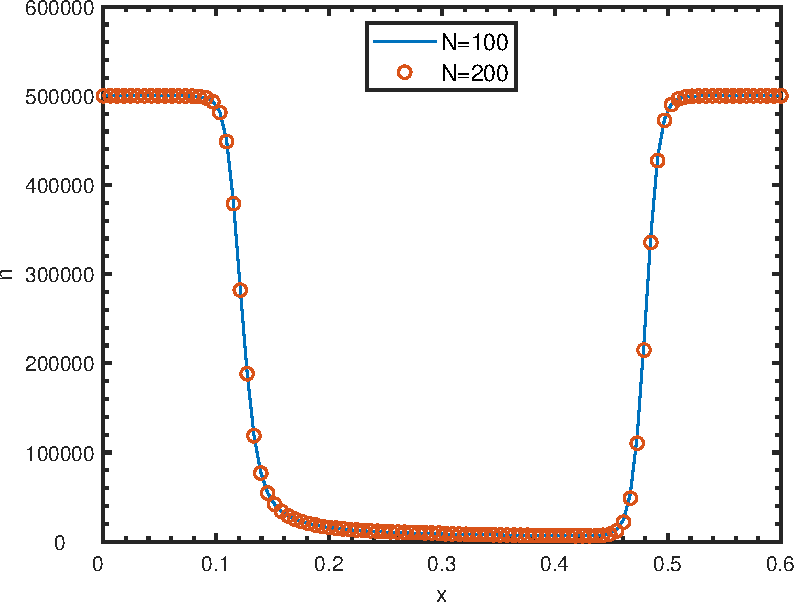
\includegraphics[width=\linewidth]{figure/DDTVDRK3Degree2mu0.75Nn.pdf}
    \end{minipage}
    \hspace{1cm}
    \begin{minipage}{0.45\linewidth}
        \centering
        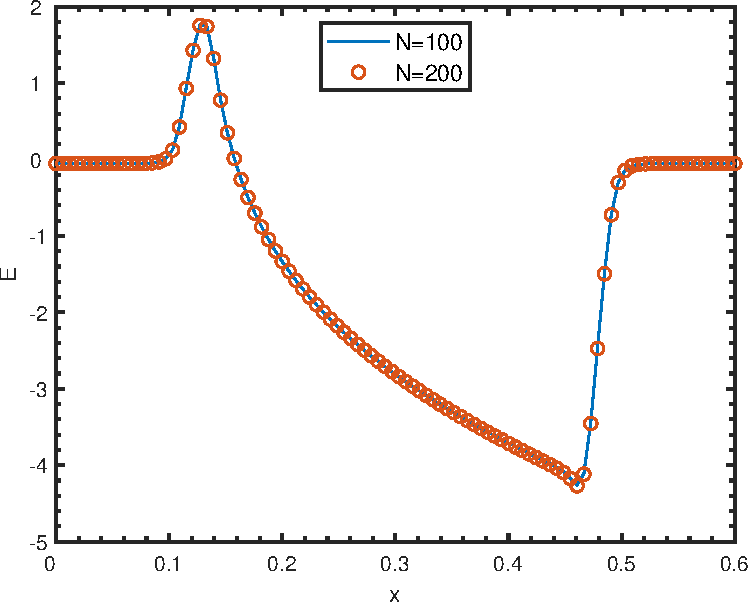
\includegraphics[width=\linewidth]{figure/DDTVDRK3Degree2mu0.75NE.pdf}
    \end{minipage}

    \centering
    \begin{minipage}{0.45\linewidth}
        \centering
        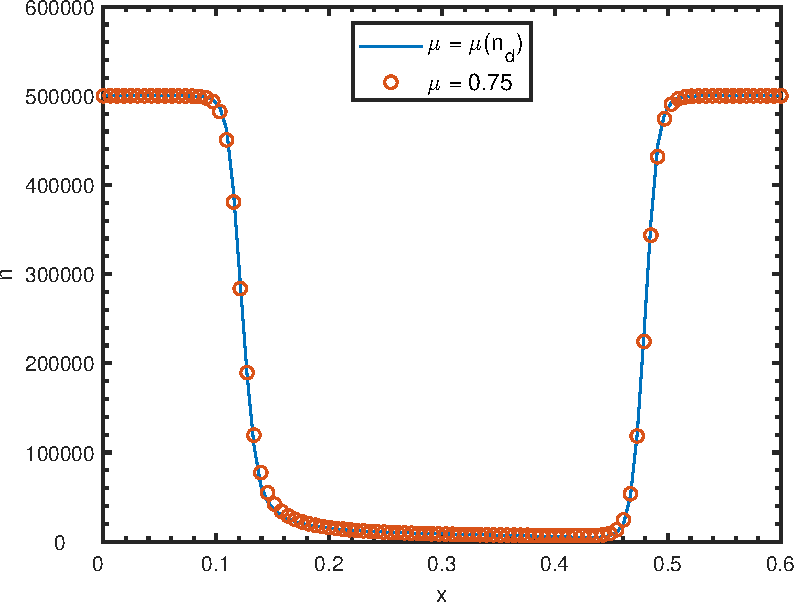
\includegraphics[width=\linewidth]{figure/DDTVDRK3Degree2N100mun.pdf}
    \end{minipage}
    \hspace{1cm}
    \begin{minipage}{0.45\linewidth}
        \centering
        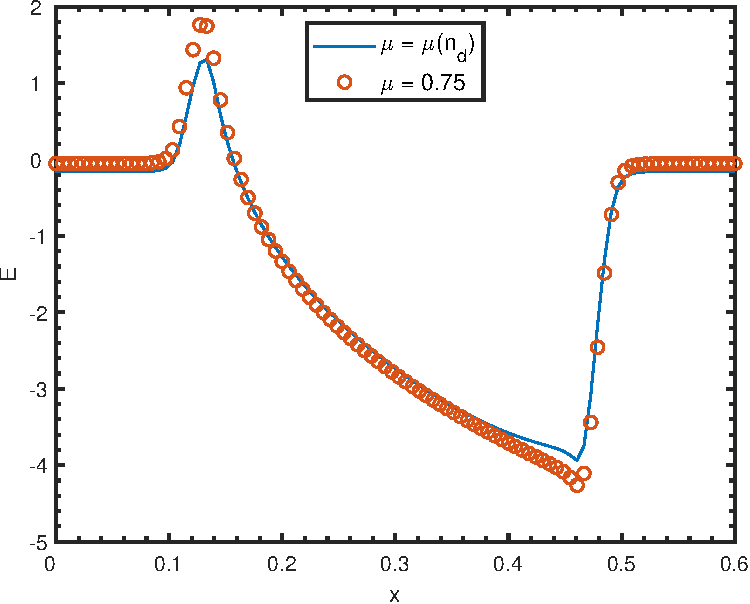
\includegraphics[width=\linewidth]{figure/DDTVDRK3Degree2N100muE.pdf}
    \end{minipage}

    \centering
    \begin{minipage}{0.45\linewidth}
        \centering
        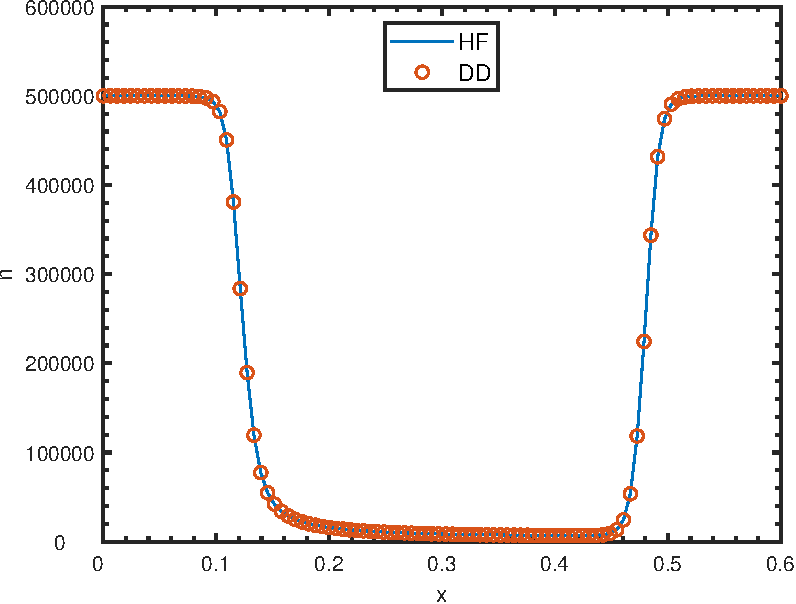
\includegraphics[width=\linewidth]{figure/DDTVDRK3Degree2N100mu0.75modeln.pdf}
    \end{minipage}
    \hspace{1cm}
    \begin{minipage}{0.45\linewidth}
        \centering
        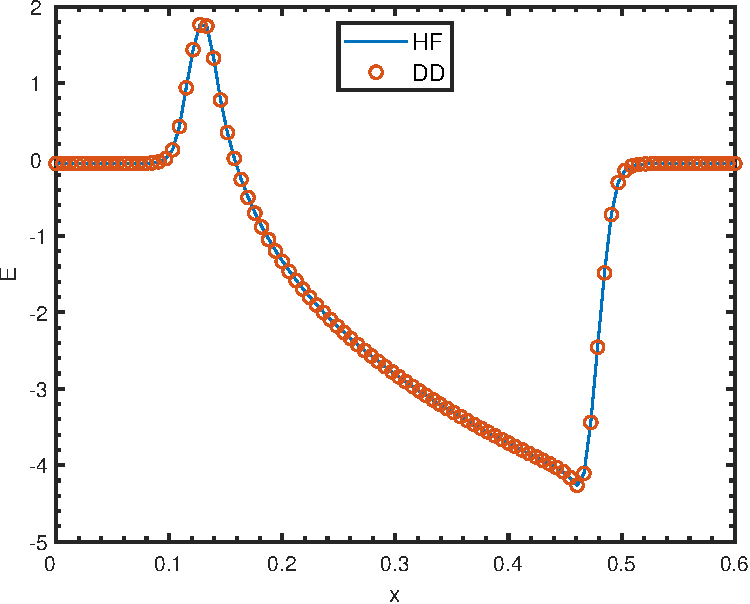
\includegraphics[width=\linewidth]{figure/DDTVDRK3Degree2N100mu0.75modelE.pdf}
    \end{minipage}
    \caption{默认值:DD模型三阶TVDRK,计算空间$V^2$,网格数$N=100$,迁移率$\mu=0.75$。左:电子浓度n;右:电势E。参数:上,网格数N;中,迁移率$\mu$;下,模型类型。}
    \label{fig:TVDRK}
\end{figure}

由于篇幅限制,这里只给出DD模型在网格数$N=100$和$N=200$情况下的全变差变化图,如\autoref{fig:TVDRKTV}所示,可以看到在一定误差范围内,总变差基本满足总变差不增。
\begin{figure}
    \centering
    \begin{minipage}{0.45\linewidth}
        \centering
        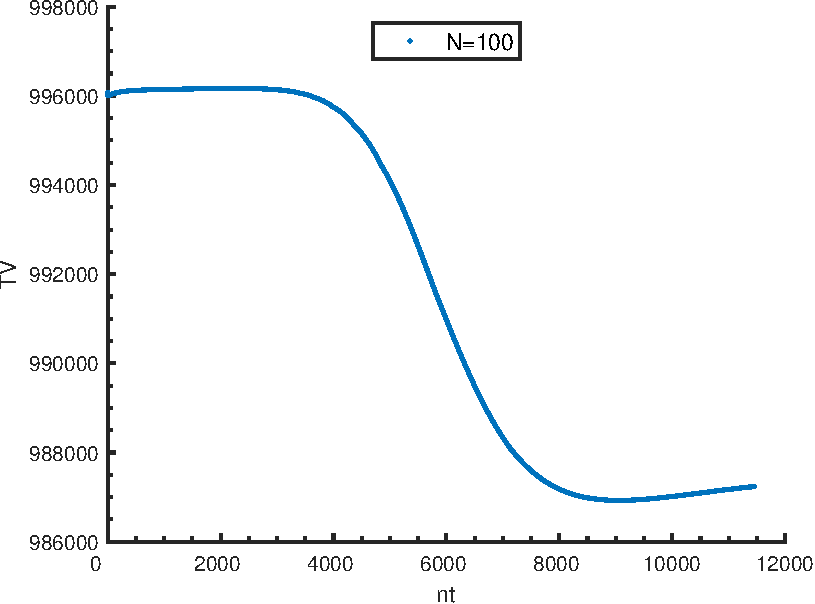
\includegraphics[width=\linewidth]{figure/TVDRKN100.pdf}
    \end{minipage}
    \hspace{1cm}
    \begin{minipage}{0.45\linewidth}
        \centering
        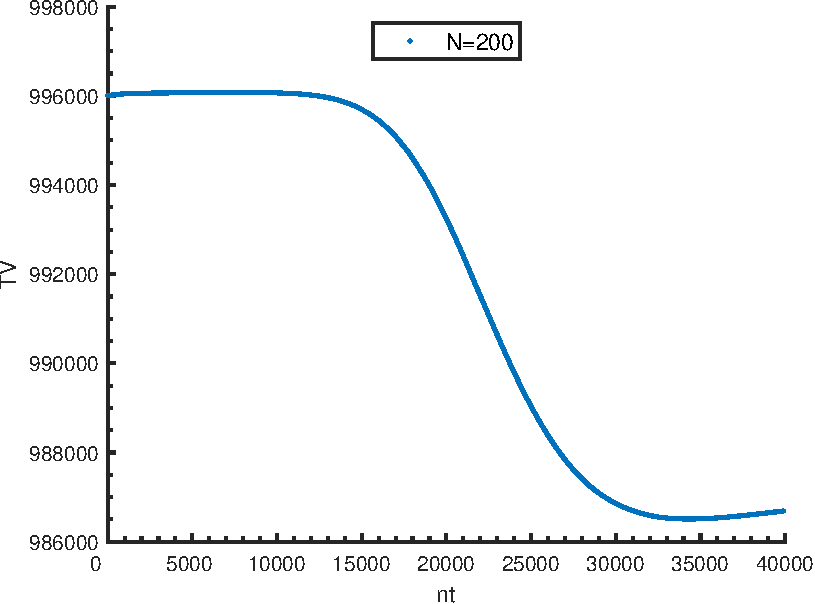
\includegraphics[width=\linewidth]{figure/TVDRKN200.pdf}
    \end{minipage}
    \caption{默认值:DD模型三阶TVDRK,计算空间$V^2$,网格数$N=100$和$N=200$,迁移率$\mu=0.75$。nt:时间层;TV:全变差。}
    \label{fig:TVDRKTV}
\end{figure}

\autoref{fig:TVDRKLimiter}是添加了改进后的minmod限制器和无添加minmode限制器的图像,由于我们的解具有良好光滑性,同时计算空间选择为$V^2$,因此是否添加限制器基本上不会产生影响。
\begin{figure}
    \centering
    \begin{minipage}{0.45\linewidth}
        \centering
        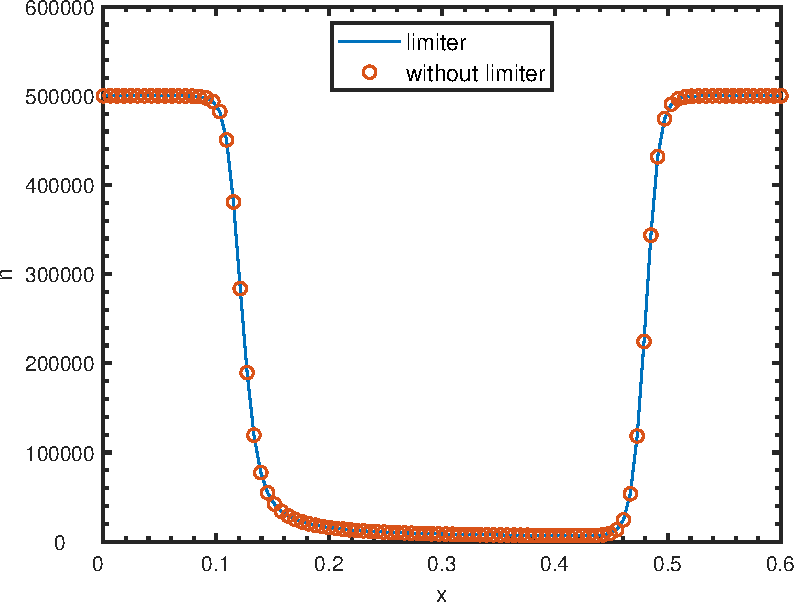
\includegraphics[width=\linewidth]{figure/DDTVDRK3Degree2N100mu0.75limitern.pdf}
    \end{minipage}
    \hspace{1cm}
    \begin{minipage}{0.45\linewidth}
        \centering
        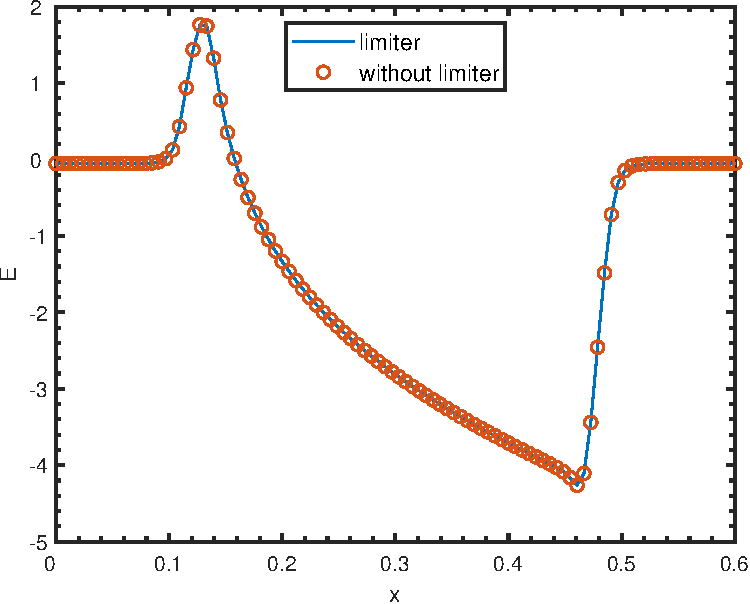
\includegraphics[width=\linewidth]{figure/DDTVDRK3Degree2N100mu0.75limiterE.pdf}
    \end{minipage}
    \caption{默认值:DD模型三阶TVDRK,计算空间$V^2$,网格数$N=100$,迁移率$\mu=0.75$。左:电子浓度n;右:电势E。}
    \label{fig:TVDRKLimiter}
\end{figure}
但如果我们的计算空间选择$V^k , k\geq 3$,如果直接让三次基函数项的系数直接取零,在数值模拟过程中仅在数个时间层后就出现了明显的误差。一般来讲,直接让三次项的系数保持不变即可,但考虑到本文模型假定了解具有良好的光滑性,又构造出了足够光滑的初始函数,不需要限制器也可以正确模拟。因此对于限制器更深入的讨论,可以在未来分析具有强震荡解的模型时再详细研究。

\subsection{IMEX LDG格式}
由于没有准确解的显式表达式,我们采取细网格上的数值解来代替真实解。
我们取网格数$N=3200$、时间步长$t=1.2e-3$和计算空间$V_h^2$的数值解作为真实解,我们有\autoref{tab:IMEXLDGerror:2}和\autoref{tab:IMEXLDGerror:3}的误差估计,其中,我们有几点要说明的地方,表中所有案例的时间步长均选择$\Delta t = 1.2e-3$,由于\eqref{eq:IMEX:es:3}中时间项相对于空间项很小,因此我们在计算精度时忽略了时间项,\autoref{tab:IMEXLDGerror:3}中第一列采用的真实解取的是网格数$N=3200$、时间步长$t=1.2e-3$和计算空间$V_h^2$的数值解,以增加更多方面的对比。在从表中数据我们可以看到,对于计算空间$V^0, V^1, V^2$我们分别得到了一阶、二阶、三阶精度。而对于从网格数$N=25$到网格数$N=50$这两个网格上求得误差明显差于更细的网格,可能的原因是因为当网格过粗时,投影得到的初值函数误差过大。此外注意到,对于随着网格加密,我们的时间步长保持不变,但依然可以得到收敛的结果,这证明了IMEX方法的无条件稳定性。在我们的验证中,$t=1.2e-3$是一个接近临界的时间步长,当选取更大的时间步长如$t=3.0e-3$时,我们的数值解随着迭代的进行很快就发散了,更精确的时间步长可以通过二分法逐渐求出,这不是本文讨论的重点,同时为了节省算力,此处不做过多展开。
\begin{table}
    \begin{tabularx}{\textwidth}{@{} *7{X} @{}}
        \toprule
            & \multicolumn{2}{c}{$V^0$} & \multicolumn{2}{c}{$V^1$} & \multicolumn{2}{c}{$V^2$}                                                     \\
        \cmidrule(lr){2-3} \cmidrule(lr){4-5} \cmidrule(lr){6-7}
        N   & $\frac{||n_h-n||}{||n||}$ & Order                     & $\frac{||n_h-n||}{||n||}$ & Order     & $\frac{||n_h-n||}{||n||}$ & Order     \\
        \midrule
        25  & 9.94e-02                  & \text{——}                 & 3.24e-02                  & \text{——} & 4.46e-03                  & \text{——} \\
        50  & 5.50e-02                  & 0.85                      & 9.48e-03                  & 1.77      & 1.24e-03                  & 1.84      \\
        100 & 2.80e-02                  & 0.97                      & 2.56e-03                  & 1.89      & 1.77e-04                  & 2.81      \\
        200 & 1.41e-02                  & 0.99                      & 6.78e-04                  & 1.92      & 2.43e-05                  & 2.87      \\
        400 & 6.97e-03                  & 1.02                      & 1.54e-04                  & 2.14      & 2.47e-06                  & 3.30      \\
        800 & 3.54e-03                  & 0.98                      & 3.52e-05                  & 2.13      & 2.79e-07                  & 3.15      \\
        \bottomrule
    \end{tabularx}
    \caption{二阶IMEX LDG格式误差估计。网格数N,收敛阶Order,计算空间$V^k, k=0,1,2$,相对误差$(||n_h-n||)/||n||$。}
    \label{tab:IMEXLDGerror:2}
\end{table}

\begin{table}
    \begin{tabularx}{\textwidth}{@{} *7{X} @{}}
        \toprule
            & \multicolumn{2}{c}{$V^0$} & \multicolumn{2}{c}{$V^1$} & \multicolumn{2}{c}{$V^2$}                                                     \\
        \cmidrule(lr){2-3} \cmidrule(lr){4-5} \cmidrule(lr){6-7}
        N   & $\frac{||n_h-n||}{||n||}$ & Order                     & $\frac{||n_h-n||}{||n||}$ & Order     & $\frac{||n_h-n||}{||n||}$ & Order     \\
        \midrule
        25  & 9.94e-02                  & \text{——}                 & 3.24e-02                  & \text{——} & 4.46e-03                  & \text{——} \\
        50  & 5.50e-02                  & 0.85                      & 9.48e-03                  & 1.77      & 1.24e-03                  & 1.84      \\
        100 & 2.80e-02                  & 0.97                      & 2.56e-03                  & 1.89      & 1.77e-04                  & 2.81      \\
        200 & 1.43e-02                  & 0.97                      & 6.78e-04                  & 1.92      & 2.43e-05                  & 2.87      \\
        400 & 7.07e-03                  & 1.02                      & 1.54e-04                  & 2.14      & 2.47e-06                  & 3.30      \\
        800 & 3.44e-03                  & 1.04                      & 3.52e-05                  & 2.13      & 2.78e-07                  & 3.15      \\
        \bottomrule
    \end{tabularx}
    \caption{三阶IMEX LDG格式误差估计。网格数N,收敛阶Order,计算空间$V^k, k=0,1,2$,相对误差$(||n_h-n||)/||n||$。}
    \label{tab:IMEXLDGerror:3}
\end{table}

\autoref{tab:time:100}和\autoref{tab:time:200}分别给出了在网格数$N=100$和$N=200$的条件下,TVD LDG格式和IMEX LDG格式达到稳态时的时间步长$\Delta t$,经过的时间层数$nt$以及到达稳态的时间$t$。从表中我们可以清楚地看到IMEX LDG要求的时间步长远小于TVD LDG格式,更大的时间步长大大减少了算力消耗。
\begin{table}
    \centering
    \begin{tabularx}{\textwidth}{@{} *7{X} @{}}
        \toprule
                   & \multicolumn{1}{c}{TVDRK3} & \multicolumn{5}{c}{IMEX3}                                         \\
        \cmidrule(lr){2-2} \cmidrule(lr){3-7}
        \midrule
        $\Delta t$ & 1.6e-05                    & 4.0e-04                   & 6.0e-04 & 8.0e-04 & 1.0e-03 & 1.2e-03 \\
        nt         & 11457                      & 414                       & 354     & 307     & 255     & 217     \\
        t          & 0.1833                     & 0.1656                    & 0.2124  & 0.2456  & 0.2550  & 0.2604  \\
        \bottomrule
    \end{tabularx}
    \caption{TVDRK LDG格式和IMEX LDG格式达到稳态的时间步长$\Delta t$,时间层数$nt$,时间$t$。网格数$N=100$,计算空间$V^2$。}
    \label{tab:time:100}
\end{table}
\begin{table}
    \begin{tabularx}{\textwidth}{@{} *7{X} @{}}
        \toprule
                   & \multicolumn{1}{c}{TVDRK3} & \multicolumn{5}{c}{IMEX3}                                         \\
        \cmidrule(lr){2-2} \cmidrule(lr){3-7}
        \midrule
        $\Delta t$ & 4.2e-06                    & 4.0e-04                   & 6.0e-04 & 8.0e-04 & 1.0e-03 & 1.2e-03 \\
        nt         & 39892                      & 416                       & 353     & 307     & 255     & 217     \\
        t          & 0.1675                     & 0.1664                    & 0.2118  & 0.2456  & 0.2550  & 0.2604  \\
        \bottomrule
    \end{tabularx}
    \caption{TVDRK LDG格式和IMEX LDG格式达到稳态的时间步长$\Delta t$,时间层数$nt$,时间$t$。网格数$N=100$,计算空间$V^2$。}
    \label{tab:time:200}
\end{table}

\autoref{fig:IMEX:N}直观地给出了在网格数$N=100$和$N=200$的条件下,IMEX LDG法的结果。可以看到在两个网格上我们均取得良好的结果。
\begin{figure}
    \centering
    \begin{minipage}{0.45\linewidth}
        \centering
        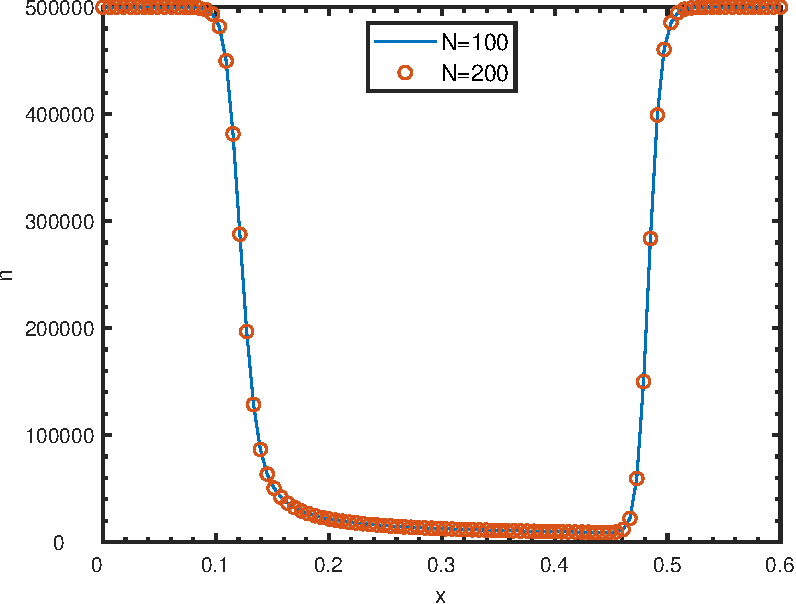
\includegraphics[width=\linewidth]{figure/IMEXNn.pdf}
    \end{minipage}
    \hspace{1cm}
    \begin{minipage}{0.45\linewidth}
        \centering
        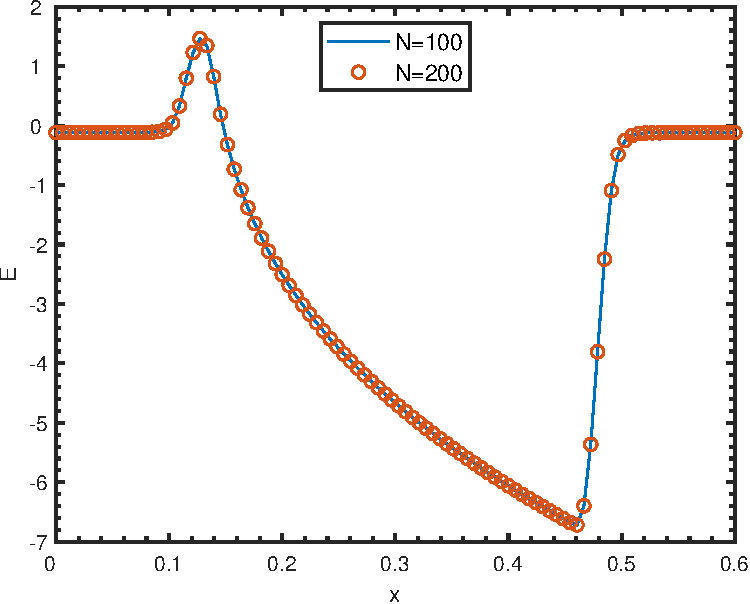
\includegraphics[width=\linewidth]{figure/IMEXNE.pdf}
    \end{minipage}
    \caption{默认值:DD模型三阶IMEXRK,计算空间$V^2$,网格数$N=100$和$N=200$,迁移率$\mu=0.75$。左:电子浓度n;右:电势E。}
    \label{fig:IMEX:N}
\end{figure}
综合上述数值算例结果,我们可以认为IMEX格式在处理如DD模型的类似的物理模型时能取得良好的结果,并有望应用于其他物理模型当中。
\section{结论与展望}
在本文,我们给出了一维漂移-扩散模型(DD)和高场模型(HF)的半离散半局部间断伽辽金(semi-LDG)格式,即对于电子浓度方程采用LDG格式,而对于电势方程采用直接积分法或者连续伽辽金有限元方法。两个模型中都包含一阶导对流项和二阶导扩散项。时间离散上我们采用全变差不增龙格-库塔法(TVDRK)。当使用k次分段多项式函数($P^k$)作为我们的计算空间,我们有对于一维DD模型($k\geq 1$)和HF模型($k\geq 2$)都有$O(h^{k+1/2})$的误差估计\cite{liu2010error},这里我们假设我们的模型都有光滑解。我们的数值算例验证了数值解的稳定性并验证了TVD LDG格式的全变差不增性质。由于我们采用的计算空间是间断的,我们需要采用合适的数值通量来处理网格单元边界的跳跃项。尽管这种格式具有良好的稳定性,但是对于时间步长有着严格的要求,这将带来大量的计算消耗。这一问题主要来源于显式处理具有二阶导的扩散项使得我们的时间步长只能有$O(h^2)$的长度。一个方法是采用隐式法来处理扩散项中的二阶导。在本文中我们给出了一阶到三阶的隐式-显式(IMEX)龙格-库塔法,该方法的想法是采用隐式方法处理线性扩散项,采用显式方法处理非线性对流项。与讨论TVD LDG格式时相同,我们采用同样的一维DD模型,但不同的是前者只对电子浓度方程使用LDG空间离散,而讨论IMEX LDG格式时,我们对电子浓度方程和电势方程都采用LDG空间离散。对于三种精度的IMEX RK法,我们分别得到对应的IMEX LDG格式。可以证明,IMEX方法具有无条件稳定性,且对于光滑解和小于某个固定常数的时间步长都收敛。我们有与$\Delta t$有关的$O(h^{k+1})$的误差估计\cite{liu2016analysis}。在我们的数值算例中,我们验证了二阶和三阶IMEX LDG格式的收敛阶,无条件稳定性和收敛性。

在本文的数值算例中,我们采用的都是均匀网格,因此,且每个单元上的数值近似都采用的时相同的$P^k$,这没有充分利用LDG方法的h-p自适应性。未来可以考虑对于变化剧烈的区域采用更细的网格以及更高阶的多项式近似,以期在不增加太多计算量的情况下提高我们的计算精度和效率。同时,我们也计划将这种方法推广到其他半导体模型。
